\documentclass[11pt]{article}
\usepackage[margin = 1in]{geometry}
\usepackage{amsmath}
\usepackage{amssymb}
\usepackage{amsthm} % for proof environment
\usepackage{enumitem}
\usepackage{graphicx}
\usepackage{indentfirst}
\usepackage{caption}
\usepackage{lscape}
\usepackage{multirow}
\usepackage{array}
\usepackage{tikz}
\usetikzlibrary{calc} % for positioning tikz nodes

\renewcommand{\labelenumii}{\arabic*)}

\tikzset{%
	hollow/.style = {circle,draw,inner sep=1.5},
	solid/.style = {circle,draw,inner sep=1.5,fill=black}%
}

\begin{document}
\begin{flushleft}
	Nick Hoffman \\
	Game Theory, Spring 2020 A \\
	Assignment 2 \\
\end{flushleft}

\begin{enumerate}
	\item Proposition: subgame-perfect equilibria exist in finite multi-stage games.
	\begin{proof}
		The proof proceeds by backwards induction. Let $ K + 1 < \infty $ be the number of stages in the game, denoting the first stage as stage 0. The game at history $ h^K $, then, consists of a finite one-shot game, which has a Nash Equilibrium by the Nash existence theorem. Moving backwards to history $ h^{K - 1} $, then, we can replace the stage $ K $ game with the payoffs from its Nash Equilibrium strategy. As in $ h^K $, the subgame at $ h^{K - 1} $ has a Nash Equilibrium. This process of backwards induction can be repeated back through stage 0. The resulting profile of strategies will be such that its restriction to any subgame in any history is a Nash Equilibrium, and thus will be a subgame-perfect equilibrium. 
	\end{proof}

	\item Player 2 chooses $ x_2 \in \{0,1\} $, and receives transfer $ p\in \{0,1\} $ from player 1. Player 2 wishes to maximize his payoff less his cost, which is 0 if $ x_2 = 0 $, and $ 1/2 $ if $ x_2 = 1 $. Player one only makes the transfer after observing $ x_2 $, and wishes to minimize $ 2(x_2 - 1)^2 - p $. Player one has the option to announce a transfer rule \emph{before} observing $ x_2 $. 
	\begin{enumerate}
		\item The decision tree for the case in which the decision rule is \emph{not} binding is:
		
		\begin{figure}[h]
			\centering
			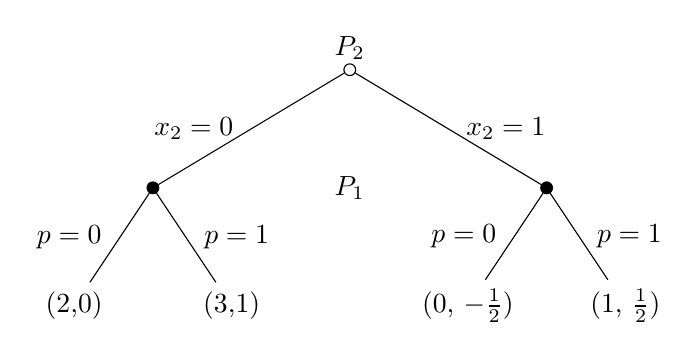
\begin{tikzpicture}
			
			\node(0)[hollow]{}
			[sibling distance=50mm]
			child{node[solid]{}
				[sibling distance=20mm]
				child{node{(2,0)}edge from parent node[left,xshift=-3]{$p = 0$}}
				child{node{(3,1)}edge from parent node[right,xshift=3]{$p = 1$}}
				edge from parent node[left,xshift=-3]{$x_2 = 0$}	
			}
			child{node[solid]{}
				[sibling distance=20mm]
				child{node{(0, $ -\frac{1}{2} $)}edge from parent node[left,xshift=-3]{$p = 0$}}
				child{node{(1, $ \frac{1}{2} $)}edge from parent node[right,xshift=3]{$p = 1$}}
				edge from parent node[right,xshift=3]{$x_2 = 1$}
			};
			\node[above]at(0){$ P_2 $};
			\node at($(0-1)!.5!(0-2)$){$ P_1 $};
			\end{tikzpicture}
		\end{figure}
	If the rule is not binding, the $ P_1 $ chooses his best response, which is always $ p = 0 $. The subgame-perfect equilibrium is 
	\begin{align*}
	P_1&: p = 0,\text{ } p = 0 \\
	P_2&: x_2 = 0
	\end{align*}
	And the payoff is $ (2,0) $
	
	\item If the decision rule $ p(x_2) $ is binding, then player 1 can induce a better outcome for herself. The rule is announced as follows:
	\[p = \begin{cases}
	0 & \text{if $ x_2 = 0 $}\\
	1 & \text{if $ x_2 = 1 $}
	\end{cases}\]
	With this binding rule in place, the tree is reduced to a simple decision for player 2:
	\newpage
	\begin{figure}[!ht]
		\centering
		\begin{tikzpicture}
		
		\node(0)[hollow]{}
		[sibling distance=50mm]
		child{node[solid]{}
			[sibling distance=20mm]
			child{node{(2,0)}edge from parent node[left,xshift=-3]{$p = 0$}}
			edge from parent node[left,xshift=-3]{$x_2 = 0$}	
		}
		child{node[solid]{}
			[sibling distance=20mm]
			child{node{(1, $ \frac{1}{2} $)}edge from parent node[right,xshift=3]{$p = 1$}}
			edge from parent node[right,xshift=3]{$x_2 = 1$}
		};
		\node[above]at(0){$ P_2 $};
		\node at($(0-1)!.5!(0-2)$){$ P_1 $};
		\end{tikzpicture}
	\end{figure}

	The subgame-perfect equilibrium is now $ P_2: x_2 = 1 $, $ P_1: p = 0, \text{ }p = 1 $, and the payoffs are $ (1, \frac{1}{2} ) $. By announcing the binding rule, Player one has made herself better off. 
	\end{enumerate}

	\item In the $ I $-player Rubinstein game, wherein all players have common discount factor $\delta$, the strategy of player $ i $ offering division 
	\[\left(\frac{1}{1 + \delta + \dots + \delta^{I - 1}}, \frac{\delta}{1 + \delta + \dots + \delta^{I - 1}}, \dots, \frac{\delta^{I - 1}}{1 + \delta + \dots + \delta^{I - 1}} \right)\]
	for all players $ i $, $ i = 1, \dots, I - 1 $ at each date $ (kI + i) $, and all other players accepting, is a subgame-perfect equilibrium. To verify, we use the one-stage deviation principle. There are three cases:
	\begin{enumerate}[label = \Roman{*}. ]
		\item On his turn, player $ i $ deviates by proposing \[x_i > \frac{\delta^{i - 1}}{\sum_{k = 0}^{I - 1} \delta^k}\]
		Because all other players follow the equilibrium strategy, this proposal is rejected. On the next turn, player $ i + 1 $ proposes following the equilibrium strategy, and this proposition is accepted. Thus, player $ i $ receives
		\[x_i = \frac{\delta^{i}}{\sum_{k = 0}^{I - 1} \delta^k} < \frac{\delta^{i - 1}}{\sum_{k = 0}^{I - 1} \delta^k}\]
		making him worse off than if he had conformed to the equilibrium strategy.
		
		\item On his turn, player $ i $ deviates by proposing \[x_i < \frac{\delta^{i - 1}}{\sum_{k = 0}^{I - 1} \delta^k}\] In this case, one of two outcomes can occur. If this proposal makes every player better off, it is accepted, and player $ i $ receives a lesser amount than he would have had he conformed to the equilibrium strategy. Alternatively, if it makes some players worse off, it is rejected. The equilibrium strategy is proposed and accepted by player $ i+1 $ in the next round, and thus player $ i $ again receives 
		\[x_i = \frac{\delta^{i}}{\sum_{k = 0}^{I - 1} \delta^k} < \frac{\delta^{i - 1}}{\sum_{k = 0}^{I - 1} \delta^k}\]
		and thus is worse off for having deviated.
		
		\item When it is not his turn to propose, player $ i $ deviates by rejecting 
		\[x_i = \frac{\delta^{i - 1}}{\sum_{k = 0}^{I - 1} \delta^k}\]
		The game then turns to the next player, which may or may not be player $ i $. The next player proposes the equilibrium strategy, which is accepted. Thus, player $ i $'s payoff for deviating is once again 
		\[x_i = \frac{\delta^{i}}{\sum_{k = 0}^{I - 1} \delta^k} < \frac{\delta^{i - 1}}{\sum_{k = 0}^{I - 1} \delta^k}\]
	\end{enumerate}
	Therefore, by the one-stage deviation principle, the strategy outlined above is the subgame-perfect equilibrium. 
	
	\item The payoffs in this game are
	\begin{table}[!htbp]
		\centering
		\setlength{\extrarowheight}{2pt}
		\begin{tabular}{cc|c|c|c|}
			& \multicolumn{1}{c}{} & \multicolumn{1}{c}{$A$}  & \multicolumn{1}{c}{$B$} & \multicolumn{1}{c}{$ C $} \\\cline{3-5}
			& $A$ & $ 4,4 $ & $ 3,0 $ & $ 1,0 $\\\cline{3-5}
			& $B$ & $ 0,3 $ & $ 2,2 $ & $ 1,0 $\\\cline{3-5}
			& $C$ & $ 0,1 $ & $ 0,1 $ & $ 1,0 $\\\cline{3-5}
		\end{tabular}
	\end{table}
	\begin{enumerate}
		\item The set of feasible payoffs is shown in Figure:
		
		\item The set of feasible and individually rational payoffs is shown in Figure:
	\end{enumerate}
\end{enumerate}

\end{document}